\PassOptionsToPackage{utf8}{inputenc}
\documentclass{bioinfo}

\usepackage{makecell}

\usepackage{floatrow}

\usepackage{comment}

\usepackage{siunitx}

% singlelinecheck=false puts subcaptions on the left
\usepackage[singlelinecheck=false]{subcaption}

\usepackage{amsthm}
\theoremstyle{definition}
\newtheorem{definition}{Definition}[section]
\newtheorem{theorem}{Theorem}[section]
\newtheorem{corollary}{Corollary}[theorem]
\newtheorem{lemma}[theorem]{Lemma}

\usepackage{amsfonts}
\usepackage{booktabs}

\usepackage{algorithm2e}
\usepackage[usenames,dvipsnames]{xcolor}
\SetAlgoLined
\usepackage{bm}

% we squeeze our figures even more together
\captionsetup{belowskip=-2pt}

\SetAlgoLined
\SetKwProg{MyStruct}{Struct}{ contains}{end}

\newcommand{\vocab}{\textbf}
\newcommand{\red}[1]{{\textcolor{Red}{#1}}}
\newcommand{\FIXME}[1]{\red{[FIXME: #1]}}

\usepackage{orcidlink}
\hypersetup{hidelinks}
\usepackage{appendix}
\newcommand{\description}{}
\usepackage[inline]{enumitem}

% table stuff
\usepackage{amsfonts}
\usepackage{booktabs}
\usepackage{siunitx}
\newcommand{\ra}[1]{\renewcommand{\arraystretch}{#1}}
\usepackage{float}
\floatstyle{plaintop}
\restylefloat{table}


\def\labelitemi{--}

\copyrightyear{2023} \pubyear{XXXX}

\access{Advance Access Publication Date: Day Month Year}
\appnotes{Genome Analysis}

\begin{document}
    \firstpage{1}

    \subtitle{Genome Analysis}

    %\title[Pangenome graph layout by HOGWILD! Path-Guided Stochastic Gradient Descent]{Pangenome graph layout by HOGWILD! Path-Guided Stochastic Gradient Descent}
    \title[Pangenome graph layout by Path-Guided Stochastic Gradient Descent]{Pangenome graph layout by Path-Guided Stochastic Gradient Descent}
    %\title[Unveiling genome variation by sequence-guided pangenome graph layouts]{Unveiling genome variation by sequence-guided pangenome graph layouts}
    %\title[PG-SGD: sequence-guided pangenome graph layouts]{PG-SGD: sequence-guided pangenome graph layouts}
    %\title[Genome-guided pangenome graph layouts via Stochastic Gradient Descent]{Genome-guided pangenome graph layouts via Stochastic Gradient Descent}
	%\title[Sequence-guided pangenome graph layouts via Stochastic Gradient Descent]{Sequence-guided pangenome graph layouts via Stochastic Gradient Descent}
    %\title[Genome-guided pangenome graph layouts]{Genome-guided pangenome graph layouts}
	%\title[Sequence-guided pangenome graph layouts]{Sequence-guided pangenome graph layouts}
    
	\author[Heumos, Guarracino \textit{et~al}.]{
        Simon~Heumos\,$^{\orcidlink{0000-0003-3326-817X}1,2,\dagger}$,
        Andrea~Guarracino\,$^{\orcidlink{0000-0001-9744-131X}3,4,\dagger}$,
        Jan-Niklas Manuel Schmelzle\,$^{\orcidlink{0000-0001-8566-4049}5,6}$,
        Jiajie Li\,$^{\orcidlink{0000-0002-9467-0659}6}$,
        Zhiru Zhang\,$^{\orcidlink{0000-0002-0778-0308}6}$,
        Sven Nahnsen\,$^{\orcidlink{0000-0002-4375-0691}1,2}$,
        Pjotr Prins\,$^{\orcidlink{0000-0002-8021-9162}3}$,
        Erik~Garrison\,$^{\orcidlink{0000-0003-3821-631X}\text{\sfb 3},*}$
    }

    \address{
        $^1$Quantitative Biology Center (QBiC), University of Tübingen, Tübingen 72076, Germany \\
        $^2$Biomedical Data Science, Department of Computer Science, University of Tübingen, Tübingen 72076, Germany \\
        $^3$Department of Genetics, Genomics and Informatics, University of Tennessee Health Science Center, Memphis, TN 38163, USA \\
        $^4$Genomics Research Centre, Human Technopole, Milan 20157, Italy \\
        $^5$Department of Computer Engineering, School of Computation, Information and Technology (CIT), Technical University of Munich, Munich 80333, Germany \\
        $^6$School of Electrical and Computer Engineering, Cornell University, Ithaca, NY 14853, USA \\
    }

    \corresp{
        $^\ast$To whom correspondence should be addressed. \\
        $^{\dagger}$The authors wish it to be known that, in their opinion, the first two authors should be regarded as Joint First Authors.\
    }

    \history{Received on XXXXX; revised on XXXXX; accepted on XXXXX}

    \editor{Associate Editor: XXXXXXX}

	\abstract{
	\textbf{Motivation:}
	The increasing availability of complete genomes demands models to study genomic variability within entire populations.
	Pangenome graphs can represent the full genetic diversity between multiple genomes, but their layouts may exhibit complex structures due to common, nonlinear patterns of genome variation and evolution.
	These structures introduce difficulty in downstream analyses, visualization, and interpretation. \\
	\textbf{Results:}
	To address these challenges, we propose a novel graph layout algorithm, the Path-Guided Stochastic Gradient Descent (PG-SGD).
	PG-SGD uses the genomes, represented in the pangenome graph as paths, to move pairs of nodes in parallel by applying a modified HOWGWILD! strategy.
	We show that our implementation efficiently computes the layout of gigabase-scale pangenome graphs, revealing their biological features. \\
	\textbf{Availability:}
	PG-SGD has been integrated in \textit{ODGI} which is released as free software under the MIT open source license.
	Source code is available at \url{https://github.com/pangenome/odgi}. \\% and documentation at \url{https://odgi.readthedocs.io/en/latest/rst/tutorials/sort_layout.html}. \\
	\textbf{Contact:} \href{egarris5@uthsc.edu}{egarris5@uthsc.edu} \\
	\textbf{Supplementary information:} Supplementary data are available at \textit{Bioinformatics} online.
	}
	
	\maketitle
	
	\section{Introduction}
	Reference genomes are the most widely used resource in genetics, serving as a foundation for a variety of analyses
	such as gene annotation, read mapping, and variant detection \citep{Singh2022}.
	However, with the availability of hundreds to thousands of high quality genomes per species, this linear model has become obsolete.
	A single genome can not faithfully represent the genetic diversity of a species, leading to the reference bias problem \citep{Ballouz2019}.
	Rather, a pangenome models the entire set of genomic elements of a given population \citep{Tettelin_2008,cpang2018,Eizenga_2020, Sherman_2020}.
	Pangenomes can be represented by a sequence graph incorporating sequences as nodes and their connections as edges \citep{Hein1989}.
	These nodes are shared for identical sequences, such as homologs, paralogs, and orthologs.
	In the variation graph model \citep{Garrison:2018}, genomes are encoded as paths visiting the nodes in the graph.
	%A bidirected graph can even contain both strands of DNA as paths. \\
	
	A pangenome graph layout is the arrangement of nodes and edges in an \textit{N}-dimensional space such that a human accessible representation of genetic variation across multiple genomes can be drawn. 
	Layout algorithms aim to find suitable node coodinates in order to minimize overlapping nodes or edges, reduce edge crossings, and promote intuitive understanding by displaying the graph layout.
	One popular approach is force-directed graph drawing \citep{cheong_force-directed_2022} which produces aesthetically-pleasing layouts.
	This is prone to get stuck in local minima, but stochastic gradient descent (SGD) implementations can alleviate such a problem \citep{Zheng2019}.
	Typically, force-directed layouts are hard to compute \citep{wang_research_2014}, but the HOGWILD! SGD is a highly parallelizable, therefore scalable solution that can be applied when the optimization problem is sparse \citep{Recht2011}.
	In practice, multidimensional scaling (MDS) is applied to minimize the difference between the visual distance and theoretical graph distance.
	This can be accomplished by using pairwise node distances to minimize an energy function.
	%\FIXME{
	%	Existing layout algorithms range from simple, force-directed methods to more complex, hierarchical layouts, each presenting unique strengths and drawbacks.
	%	Force-directed methods offer an aesthetic layout based on a physics simulation but may struggle with scalability for larger graphs (XXX WE NEED CITATIONS XXX).
	%	In contrast, hierarchical layouts handle layered relationships and dependencies, yet can exhibit limitations when dealing with non-hierarchical data (XXX WE NEED CITATIONS XXX)
	%}
	Since pangenome graphs represent genomes as paths in the graph, a reasonable distance metric would be the nucleotide distance between a pair of nodes traversed by the same path.
	To our knowledge, no algorithm takes into account such biological information to compute the pangenome graph layouts.
	
	Here, we present a new pangenome graph layout algorithm which applies a path-guided stochastic gradient descent (PG-SGD) to move pairs of nodes in parallel with a modified HOGWILD! strategy.
	The algorithm computes the pangenome graph layout that best reflects the nucleotide sequences in the graph.
	PG-SGD can be extended in any number of dimensions. We provide in the ODGI toolkit \citep{Guarracino2022} implementations to produce layouts in 1 dimension (1D) and 2 dimensions (2D).
	% We may want to adjust some citations using https://tex.stackexchange.com/questions/585942/how-to-display-the-first-two-authors-in-a-citation-call-out.

	\section{Algorithm}
	%\FIXME{WE ONLY WANT TO TALK ABOUT LAYOUTS AND PRODUCING LAYOUTS, NOT ABOUT GRAPH SORTING. PG-SGD PRODUCES 1D AND 2D LAYOUTS. IN 1D WE SORT A GRAPH BY PROJECTING THE ACTUAL 1D LAYOUT INTO A NODE ORDER!}
	
	PG-SGD is inspired by \cite{Zheng2019}, but we designed the algorithm to work on pangenomes in the form of a variation graph (Definition \ref{def:vg}).
	
	\begin{definition}
		\label{def:vg}
		Variation graphs are a mathematical formalism to represent pangenome graphs \citep{Garrison_2019_thesis}.
		In the variation graph $\mathcal{G} = (\mathcal{V}, \mathcal{E}, \mathcal{P})$, nodes (or vertices) $\mathcal{V} = v_1\ldots v_{|\mathcal{V}|}$ contain nucleotide sequences.
		Each node $v_i$ has a unique identifier $i$ and an implicit reverse complement $\bar{v_i}$.
		The node strand $o$ represents node orientation.
		Edges $\mathcal{E} = e_1\ldots e_{|\mathcal{E}|}$ connect ordered pairs of node strands ($e_i = ( o_a, o_b )$), defining the graph topology.
		Paths $\mathcal{P} = p_1\ldots p_{|\mathcal{P}|}$ are series of connected steps $s_i$ that refer to node strands in the graph ($p_i = s_1 \ldots s_{|p_i|}$); the paths represent the genomes embedded in the graph.
	\end{definition}

	PG-SGD's pseudocode is shown in Algorithm~\ref{alg:pg_sgd} and key steps are sketched in Figure \FIXME{Add puritan figure.}.
	In brief, the algorithm moves one pair of nodes $( v_i, v_j )$ at a time, minimizing the difference between the layout distance $ld_{ij}$ of the two nodes and the nucleotide distance $nd_{ij}$ of the same nodes as calculated along a path that traverses them.
	%Our multithreaded implementation (\url{https://odgi.readthedocs.io/en/latest/rst/tutorials/sort_layout.html}) presents a working prototype that is based on succinct graph data structures (\url{https://doi.org/ghqdzw}):
	$v_i$ is the node associated with the step $s_i$ sampled uniformly from all the steps in $\mathcal{P}$.
	$v_j$ is the node associated with the step $s_j$ sampled from the same path of $s_i$ by following a Zipfian distribution \citep{Zipf1932}.
	The difference between $nd_{ij}$ and $ld_{ij}$ guides the update of the node coordinates in the layout.
	The magnitude $r$ of the update depends on the learning rate $\mu$ of the SGD.
	The number of iterations steers the annealing step size $\eta$ which determines the learning rate $\mu$.
	%A key property of pangenome graph layouts is that their nodes can be arranged so that most edges go between nodes that are close together in the node order \citep{Guarracino2022}.
	A large $\eta$ in the first iterations leads to a globally linear (in 1D) or planar (in 2D) layout.
	By decreasing $\eta$, the layout adjustments become more localized, ensuring that the nodes are positioned in a way to best reflect the nucleotide distances in the paths (i.e., in the genomes). % LIAR: down to the single base pair level.
	
	\SetKwProg{for}{for}{:}{end}
\SetKwProg{pgsgd}{PG-SGD}{:}{end}
\SetKwProg{each}{for each}{:}{end}
\SetKwProg{IF}{if}{:}{end}

\SetKwFunction{PathIndex}{PathIndex}
\SetKwFunction{LayoutInitialization}{LayoutInitialization}
\SetKwFunction{InitZipf}{InitZipf}
\SetKwFunction{Unif}{Unif}
\SetKwFunction{Zipf}{Zipf}
\SetKwFunction{StepCount}{StepCount}
\SetKwFunction{Path}{Path}
\SetKwFunction{StepPos}{StepPos}

\begin{algorithm}
	\pgsgd{\textbf{(}$\mathcal{G}$\textbf{)}}{
		\textbf{input:} variation graph $\mathcal{G} = (\mathcal{V}, \mathcal{E}, \mathcal{P})$ \\
		%https://tex.stackexchange.com/questions/22643/how-to-write-letters-in-bold-in-the-math-mode
		\textbf{output:} $N$-dimensional layout $\mathcal{L}$ with $|\mathcal{V}|$ nodes \\
		$\mathcal{XP}$ $\gets \PathIndex(\mathcal{G})$ \tcp{for path position lookup} 
		%\boldsymbol{$Z$} $\gets ZipfZetas(G,P)$ \\ %@Andrea is this correct like this?
		$\mathcal{L}$ $\gets \LayoutInitialization(\mathcal{V}, N)$ \\ %\tcp{random or deterministic} 
		$\mathcal{Z} \gets \InitZipf(\mathcal{G},\mathcal{XP})$ \tcp{Zipfian distribution}
		% atomic positions initialization?
		% TODO for simplicity reasons I would only describe the 2D one here
		\for{$\eta$ $in$ $annealing$ $schedule$}{ %our "schedule" actually is the number paths.... we should specify this I would say
			\each{$planned$ $term$ $update$} { % I think we can remove i<j, because we don't care about that
				$s_i \gets \Unif(\mathcal{XP})$ \tcp{uniform sampling of a step from $\mathcal{P}$}
				$p \gets \Path(s_i,\mathcal{XP})$ \tcp{path of $s_i$}
				\uIf{$(cooling$ $||$ $flip)$} {
					$s_j \gets \Unif(\StepCount(p, \mathcal{XP}))$ \tcp{uniform sampling of a step from $p$}
				} \Else {
					$s_j \gets \Zipf(p)$ \tcp{Zipfian sampling of a step from $p$}
				}
				$p_i \gets \StepPos(s_i)$ \tcp{nuc. position}
				$p_j \gets \StepPos(s_j)$ \tcp{nuc. position}
				$nd_{ij} \gets ||p_i - p_j||$ \tcp{nuc. distance} %mag is nx
				$ld_{ij} \gets ||l_{i} - l_j||$ \tcp{layout distance}
				$w_{ij} \gets \frac{1.0}{nd_{ij}}$ \tcp{term weight} 
				$\mu \gets w_{ij}\eta$ \tcp{learning rate}  % current learning rate is given by term weight and step size
				\IF{$\mu>1$} {
				$\mu \gets 1$
				}
				$\delta \gets \mu \cdot \frac{ld -nd_{ij}}{2}$ \tcp{the actual delta}
				\uIf{$\delta <= 0$} {
					$STOP$ \tcp{we can't optimize more}
				}
				% TODO stop early?
				% TODO potentially store new delta max?
				$r \gets \delta - ld_{ij}$ \tcp{size of the update}
				$l_i \gets l_i - r\cdot ld_{ij}$ \tcp{update $v_i$ coordinates}
				$l_j \gets l_j - r\cdot ld_{ij}$ \tcp{update $v_j$ coordinates}
			}
		}
	}
	\caption{Pseudocode of PG-SGD.}
	\label{alg:pg_sgd}
\end{algorithm}

	%In standard SGD layout algorithms, the problem space is given by pairwise node comparisons. In PG-SGD, the problem space is given by the pairwise path step comparisons. The number of path steps in large variation graphs can be several orders of magnitude higher than the number of nodes. Therefore, the number of term updates in PG-SGD is bound to the number of path steps in the graph.
	%Should the delta of $nd_{ij}$ and $ld_{ij}$ become 0 before the annealing schedule is finished, the algorithm stops.

	Originating from empirical inspection of word frequency tables, Zipf's law states that a word with rank $n$ occurs $1/n$ times as the most frequent one.
	It's mathematical formulation is called the Zipfian distribution and its rank-frequency distribution is related to the inverse power law.
	Sampling $s_j$ from a Zipfian distribution fixed in the $s_i$'s path position space increases the possibility to draw a nucleotide position close to $s_i$.
	So there is a high chance to use small nucleotide distances $nd_{ij}$ to refine the layout of nodes comprising a few base pairs.

	To provide balance between global and local layout updates, in half of the updates ($flip$ flag in Algorithm~\ref{alg:pg_sgd}) the $s_j$ is sampled uniformly instead from a Zipfian distribution (uniform sampling favours global updates).
	Additionally, to boost the local linearity (in 1D) or planarity (in 2D) of the graph layout, a \textit{cooling} phase skewes the Zipfian distribution after half the number of iterations, so that the possibility of a a small sampled nucleotide distance is significantly increased. 

	\section{Implementation}
	
	We implemented PG-SGD in ODGI \citep{Guarracino2022}. % which serves as an interface to graphs in the GFA (\url{https://github.com/GFA-spec/GFA-spec}) format. 
	Our path index is a strict subset of the XG index~\citep{Garrison:2018} where we specifically avoid using succinct SDSL data structures \citep{Gog2014}.
	Instead, we only use bit compressed integer vectors, enabling efficient retrieval of path positions to quickly compute nucleotide distances without the need to store all pairwise distances between nodes in memory.
	This allows PG-SGD to scale on large pangenome graphs representing thousands of whole genomes.

	Graph layout initialization can significantly influence the quality of the final layout.
	In the 1D implementation, nodes are placed in the same order as they appear in the input graph by default, although support for random layout initialization is also provided.
	This random placement ensures that each run of the PG-SGD method could potentially yield a different result, thereby increasing the likelihood of obtaining a meaningful layout.
	In 2D, we offer several layout initialization techniques.
	One option is to position nodes in the first layout dimension according to their order in the input graph and to add either uniform or Gaussian noise in the second dimension.
	Another possibility is to arrange nodes along a Hilbert curve, which often favors the creation of planar final layouts.

	Our implementation is multithreaded and uses shared memory for the layout vector following the HOGWILD! strategy \citep{Recht2011}: Threads perform layout updates without any locking for additional speed up.
	This is possible because pangenome graphs are typically sparse \citep{Guarracino2022}, with low average node degree, meaning most updates only modify small parts of the entire layout.
	The HOGWILD! SGD algorithm writes the layout updates to a shared non-atomic double vector, whereas PG-SGD stores node coordinates in a vector of atomic doubles.
	Such a vector ensures that no memory overwrites are possible. Our tests revealed basically no performance loss with respect to the non-atomic counterpart.
	
    \iffalse
    Fig. 1: Describe how our approach works, especially a single update operation (Fig. \ref{fig:sketches}). Explanation of 1D graph updating in Figures \ref{fig:1d_before_update}-\ref{fig:1d_after_update}. Explanation of 2D graph updating in Figures \ref{fig:2d_before_update}-\ref{fig:2d_after_update}. Zipfian distribution.

    \begin{figure*}[!htb]
	\centering
		%\hline
		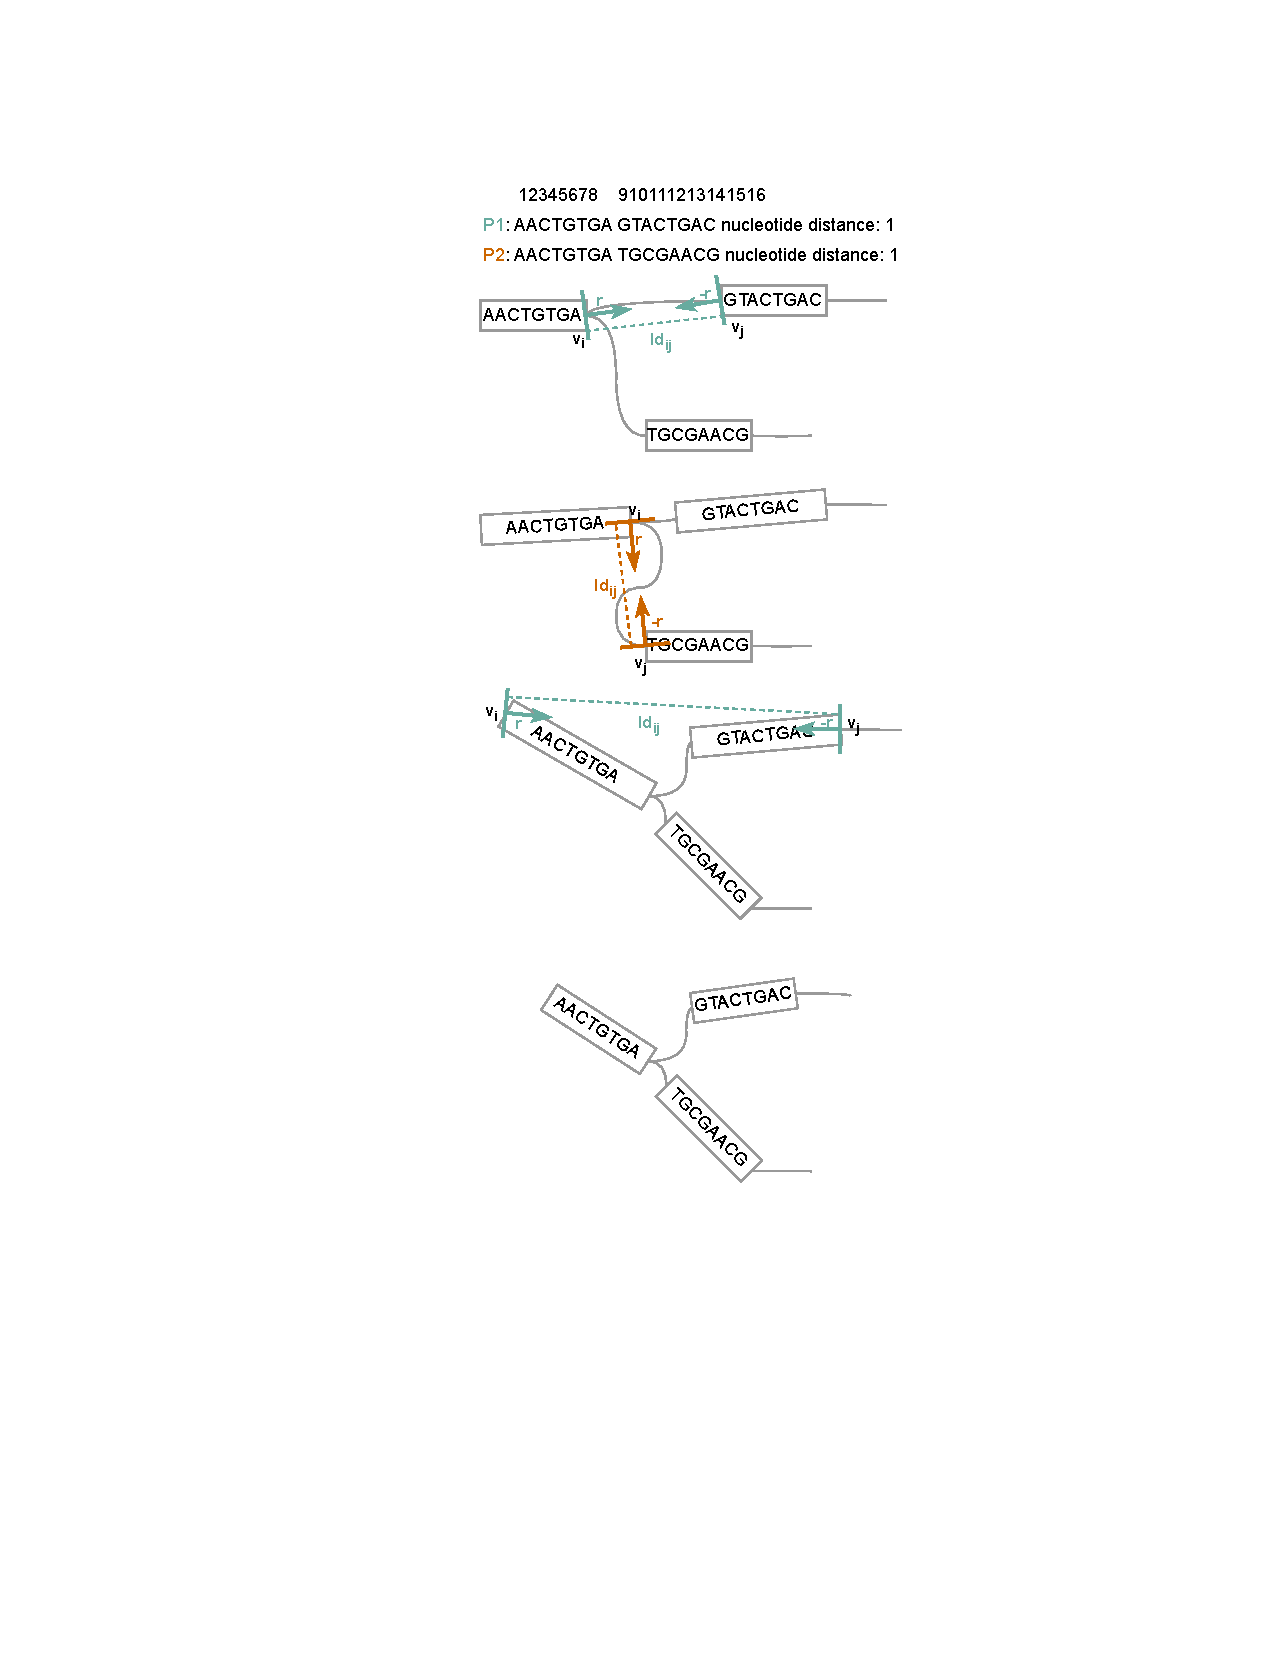
\includegraphics[width=\linewidth, trim=0cm 8cm 0cm 0cm, clip]{fig/sketches/PG-SGD.drawio.pdf}
	\caption{
		2D PG-SGD update operation sketches. \\
		\FIXME{ADD CAPTION.} \\ 
		\FIXME{PROVIDE SEVERAL NICE FIGURES SO WE CAN REARRANGE STUFF INTO SUBFIGURES.}
	}
	\label{fig:sketches}
\end{figure*}
    \fi

    \section{Results}
    \label{sec:results}

    \subsection{Performance}
	We apply PG-SGD to the recent draft human pangenome reference \citep{Liao2023} to show the scalability and practicality of the algorithm with a real pangenome.
	Experiments were conducted on a cluster with 24 \texttt{Regular} nodes (32 cores / 64 threads AMD EPYC 7343 processors with 512 GB RAM each) and 4 \texttt{HighMem} nodes (64 cores / 128 threads AMD EPYC 7513 processors with 2048 GB RAM each).
	We downloaded pangenome graphs for each autosome (24 in total) and for the mitochondrial DNA.
	Each graph represents 90 whole human haplotypes: 44 diploid individuals plus the GRCh38 \citep{Schneider2017} and CHM13 \citep{Nurk_2021} haploid human references.
	See Supplementary Table~\ref{tab:layout} for graph statistics.
	When applied to these pangenome graphs using one \texttt{Regular} node for each calculation, PG-SGD obtains the graph layouts in \FIXME{XXXX minutes/hours on average}, with the slowest chromosome being chromosome 16 (Supplementary Table~\ref{tab:layout}).
	This is expected since chromosome 16 presents one of the highest levels of segmentally duplicated sequence among the human autosomes \citep{Martin2004}.
	Repetitive sequences lead to graph nodes with a very high number of path traversals, which are computationally expensive to work with \citep{Guarracino2022}.
	Memory consumption is \FIXME{XXXX GB of RAM on average}, with the memory peak occurring with chromosome 1, the biggest one in humans.
	Given its scalability, we even applied PG-SGD to the full graph with all chromosomes together using a \texttt{HighMem} node (Supplementary Table~\ref{tab:layout}).
	Overall, PG-SGD is ~\FIXME{XX}X faster than BandageNG \FIXME{HOW TO CITE IT?}, the current state-of-the-art for graph visualization, while using ~{}X less memory.

    \subsection{Pangenome graphs layouts reveal biology features}
	Graph visualization is essential for understanding pangenome graphs and the genome variation they represent.
	We show how PG-SGD allows us quickly gain insight into biological data by looking at the graph layout structure.
	\FIXME{Describe a full chromosome and/or 1/a few selected loci, HLA, C4, beta-defensin locus, LPA, stuff from the human paper or PGR-TK.}

	% \iffalse
	% Fig. 2: Performance evaluation 1D + 2D: Time + RAM by number of haplotypes (Fig.~\ref{fig:haps_time_ram}). Time + RAM by number of threads (Fig.~\ref{fig:threads_time_ram}). Full human graph.
    % \\
    % 1D (max. threads) vs. ALIBI; we should compare time + RAM in Fig.~\ref{fig:alibi}.
    % But also by our sorting goodness metrics: odgi sort + the one suggested in the ALIBI paper in Table 1.
    % \\
    % 2D (max. threads) + odgi draw vs. Bandage in Fig.~\ref{fig:bandage}.
    % \begin{figure*}[!htb]
	\centering
	%\hline
	\begin{subfigure}[t]{0.4\textwidth}
		\centering
		\caption{}
		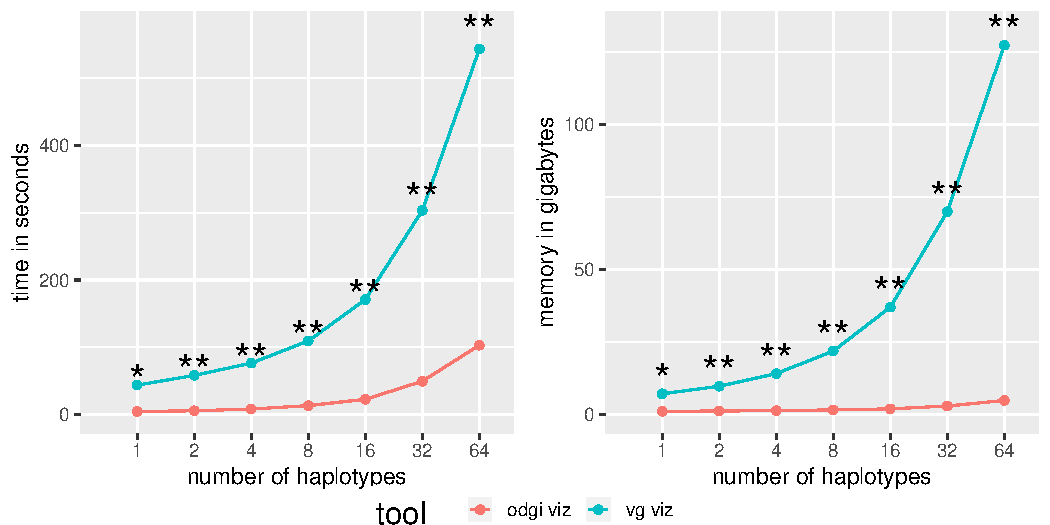
\includegraphics[width=\linewidth]{fig/performance/TODO_by_haps_eval_time_ram.pdf}
		\label{fig:haps_time_ram}
	\end{subfigure}
	\begin{subfigure}[t]{0.4\textwidth}
		\centering
		\caption{}
		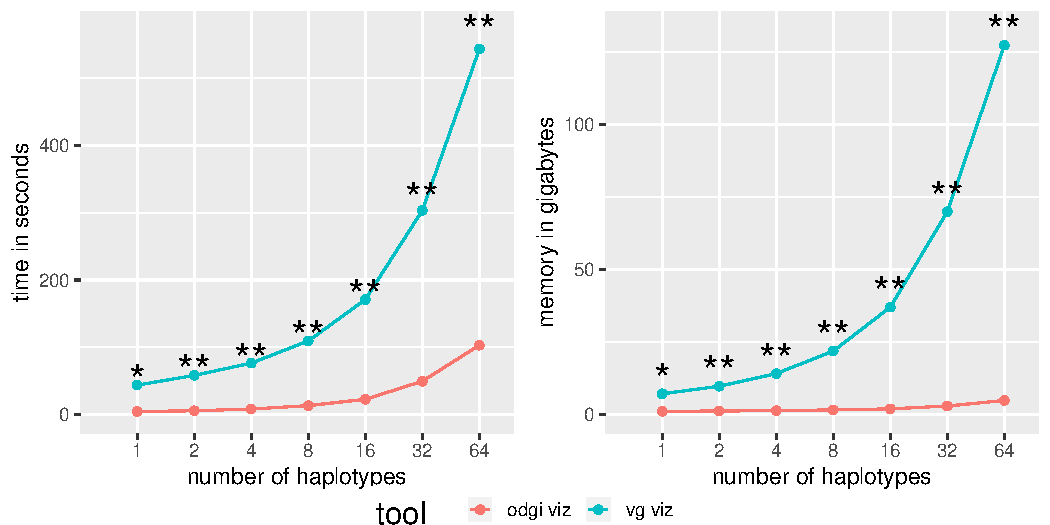
\includegraphics[width=\linewidth]{fig/performance/TODO_by_threads_eval_time_ram.pdf}
		\label{fig:threads_time_ram}
	\end{subfigure}
	%\smallskip
	\begin{subfigure}[t]{0.4\textwidth}
		\centering
		\caption{}
		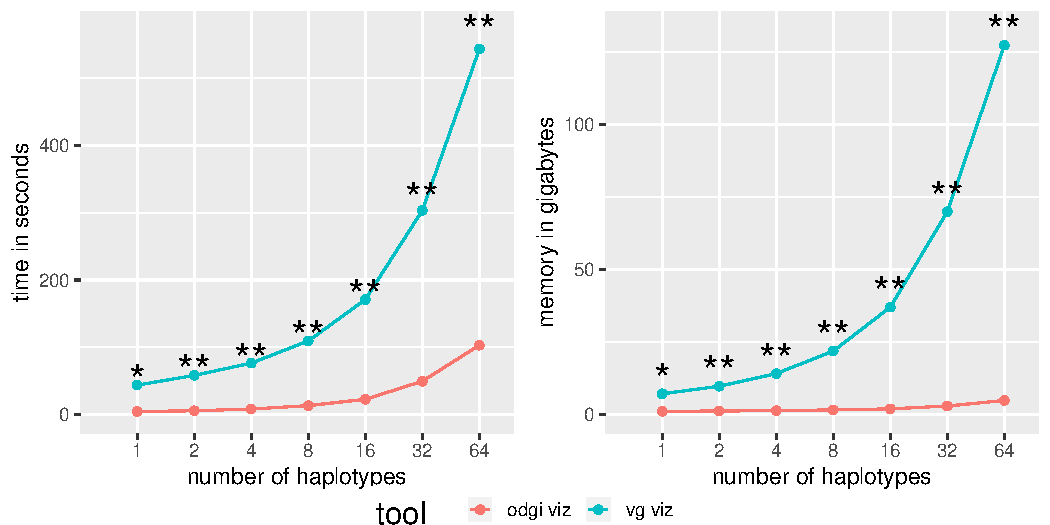
\includegraphics[width=\linewidth]{fig/performance/TODO_1d_alibi_time_ram.pdf}
		\label{fig:alibi}
	\end{subfigure}
	\begin{subfigure}[t]{0.4\textwidth}
		\centering
		\caption{}
		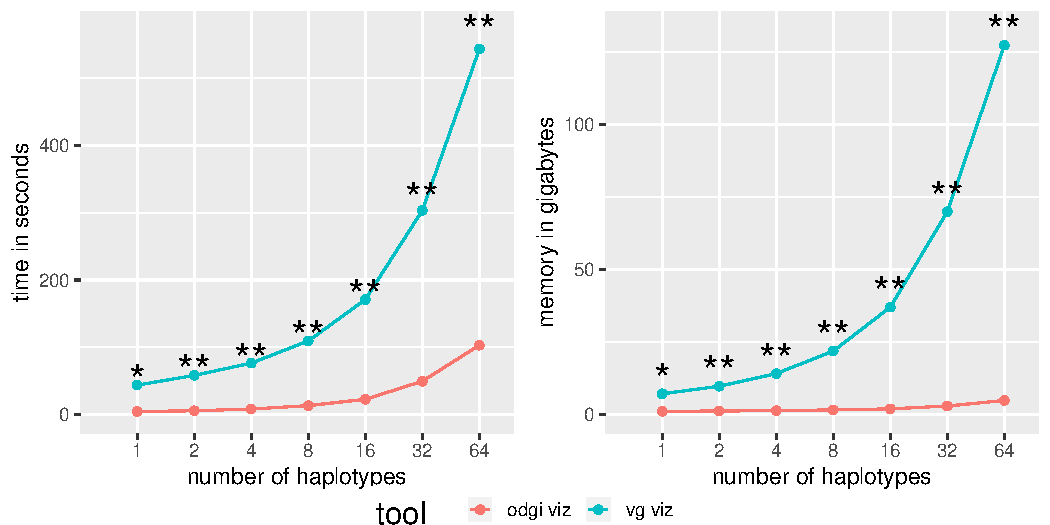
\includegraphics[width=\linewidth]{fig/performance/TODO_by_2d_draw_bandage_time_ram.pdf}
		\label{fig:bandage}
	\end{subfigure}
	\caption{
		Performance evaluations.
		\textbf{(a)} PG-SGD 1D and 2D by haplotypes. \textbf{(b)} PG-SGD 1D and 2D by threads. \textbf{(c)} PG-SGD vs. ALIBI. \textbf{(d)} PG-SGD + draw vs. BANDAGE.
	}
	\label{fig:performance}
\end{figure*}
    % \\
    % \\
    % Table 1: Metrics of the ALIBI and PG-SGD graphs from Fig. 2.
    % \begin{table}[]
	\caption{Metrics of the 1D PG-SGD and ALIBI graphs.}
	\begin{tabular}{|l|l|l|}
		\hline
		& 1D PG-SGD & ALIBI \\ \hline
		METRIC 1 &           &       \\ \hline
		METRIC 2 &           &       \\ \hline
	\end{tabular}
\end{table}
    % Already, PG-SGD outperforms existing graph linearization methods like the flow procedure (\url{https://doi.org/gdw58w}) or ALIBI (\url{https://doi.org/hkv3}).
    % \paragraph{Latent graph structure reveals underlying biology}
    % Fig. 3: Cool quantitative 1D sortings and 2D layouts: biological implications.
    % Randomly sorted. PG-SGD sorted. Ygs sorted. Reference sorted.
    % We want a pipeline of sortings. 2D layout of the whole HPRC.
    % Chr6 HPRC HLA graph? Chr8 beta-defensin gene cluster HPRC? Whole HPRC?
    % \\
    % We could also try to build a gastric cancer pangenome graph with data from \url{https://www.nature.com/articles/s41467-022-33073-7} from up to 185 samples.
    % However, we would have to request access to the data.
    % \\
    % \\
    % \begin{figure*}[!htb]
	\centering
	%\hline
	\begin{subfigure}[t]{0.4\textwidth}
		\centering
		\caption{}
		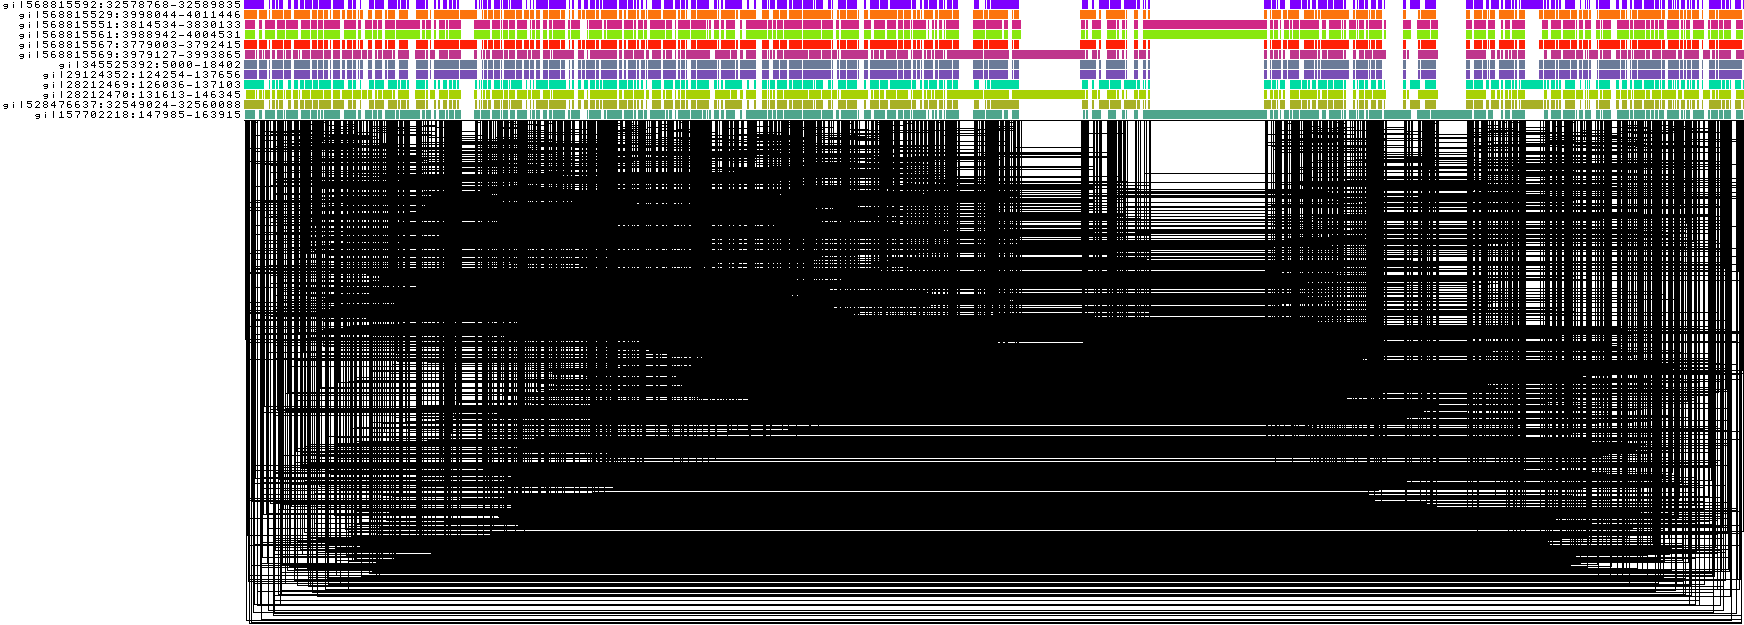
\includegraphics[width=\linewidth]{fig/latent_graph_structure/DRB1-3123.fa.gz.c666522.417fcdf.seqwish.og.r.og.png}
		\label{fig:random}
	\end{subfigure}
	\begin{subfigure}[t]{0.4\textwidth}
		\centering
		\caption{}
		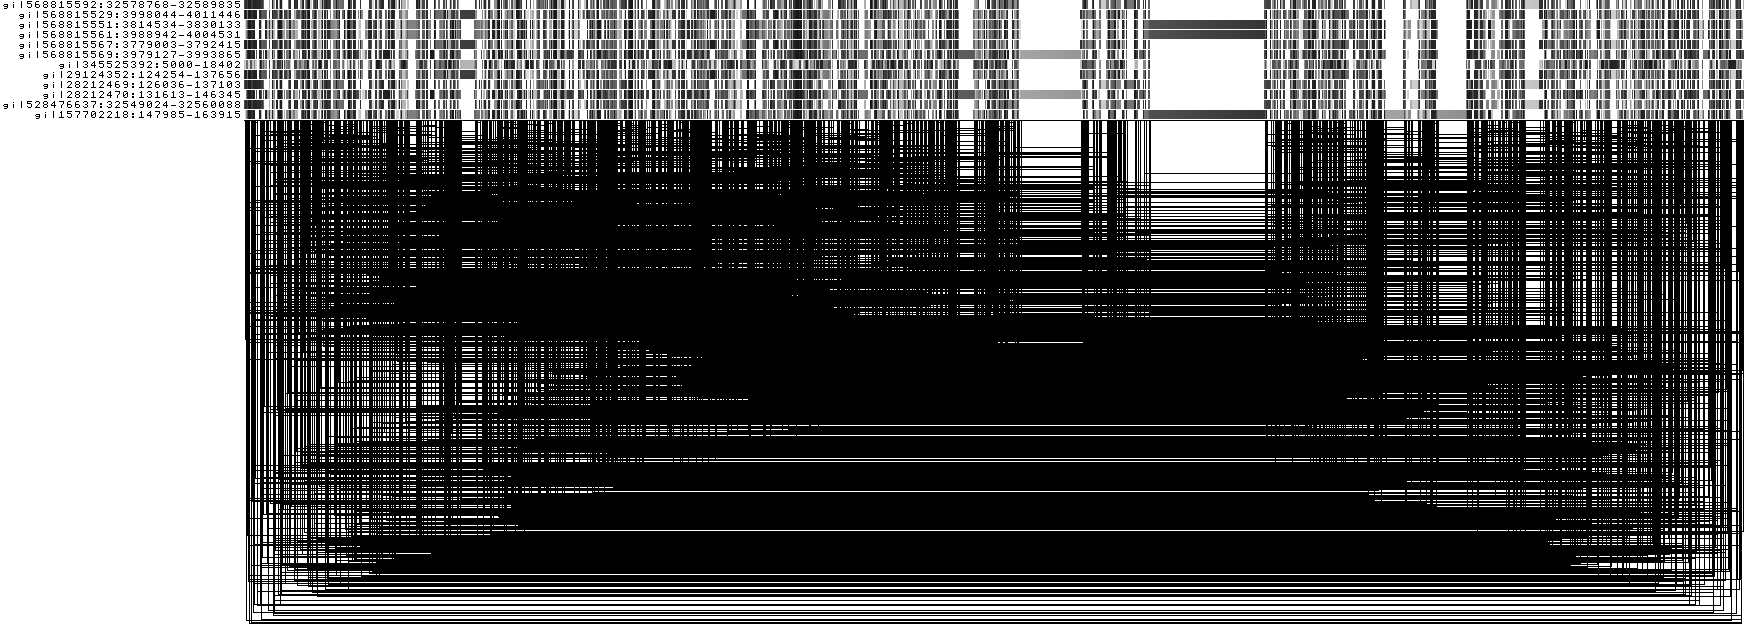
\includegraphics[width=\linewidth]{fig/latent_graph_structure/DRB1-3123.fa.gz.c666522.417fcdf.seqwish.og.r.og.ud.png}
		\label{fig:random_pos}
	\end{subfigure}
	%\smallskip
	\begin{subfigure}[t]{0.4\textwidth}
		\centering
		\caption{}
		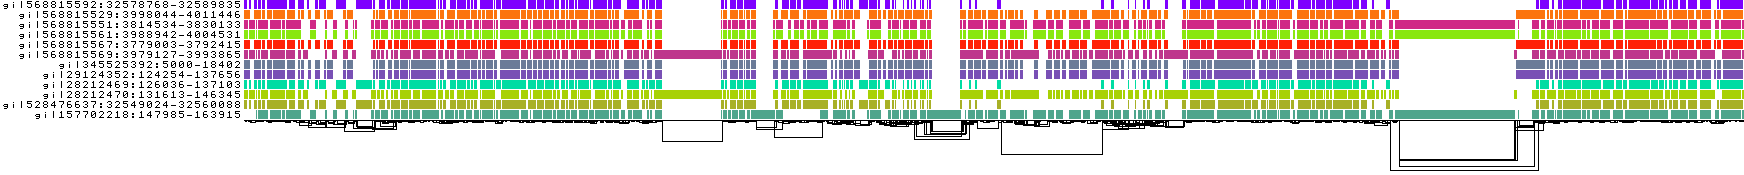
\includegraphics[width=\linewidth]{fig/latent_graph_structure/DRB1-3123.fa.gz.c666522.417fcdf.seqwish.og.Y.og.png}
		\label{fig:sorted}
	\end{subfigure}
	\begin{subfigure}[t]{0.4\textwidth}
		\centering
		\caption{}
		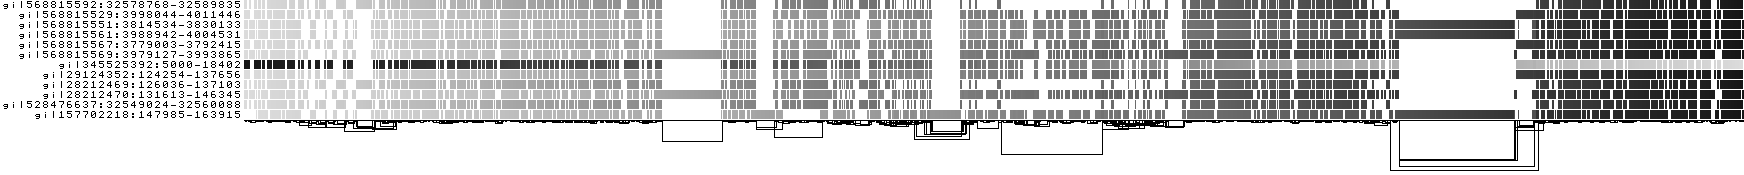
\includegraphics[width=\linewidth]{fig/latent_graph_structure/DRB1-3123.fa.gz.c666522.417fcdf.seqwish.og.Y.og.ud.png}
		\label{fig:sorted_pos}
	\end{subfigure}
	\begin{subfigure}[t]{0.4\textwidth}
		\centering
		\caption{}
		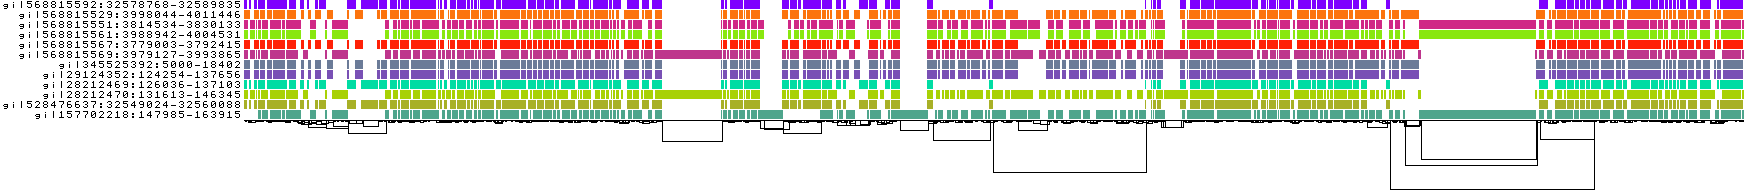
\includegraphics[width=\linewidth]{fig/latent_graph_structure/DRB1-3123.fa.gz.c666522.417fcdf.seqwish.og.Ygs.og.png}
		\label{fig:pipeline}
	\end{subfigure}
	\begin{subfigure}[t]{0.4\textwidth}
		\centering
		\caption{}
		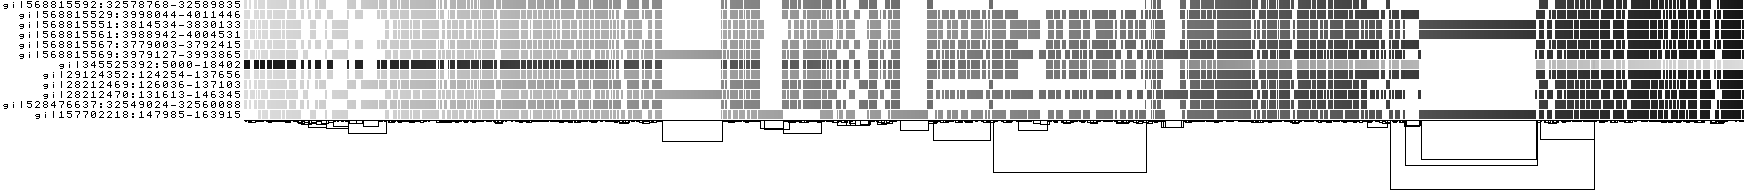
\includegraphics[width=\linewidth]{fig/latent_graph_structure/DRB1-3123.fa.gz.c666522.417fcdf.seqwish.og.Ygs.og.ud.png}
		\label{fig:pipeline_pos}
	\end{subfigure}
	\begin{subfigure}[t]{0.4\textwidth}
		\centering
		\caption{}
		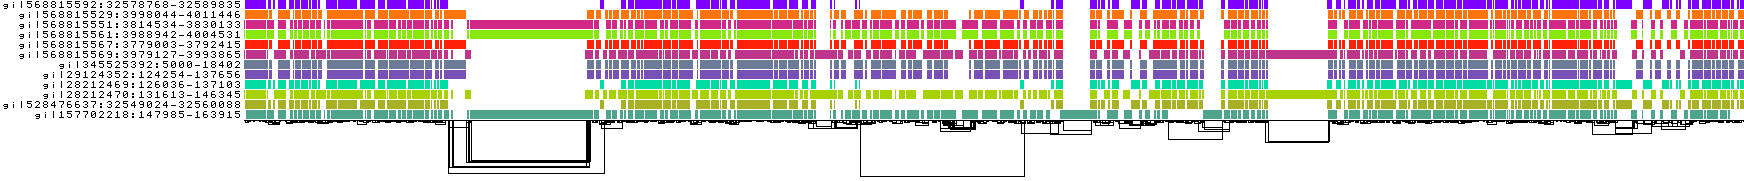
\includegraphics[width=\linewidth]{fig/latent_graph_structure/DRB1-3123.fa.gz.c666522.417fcdf.seqwish.og.YH.og.png}
		\label{fig:ref}
	\end{subfigure}
	\begin{subfigure}[t]{0.4\textwidth}
		\centering
		\caption{}
		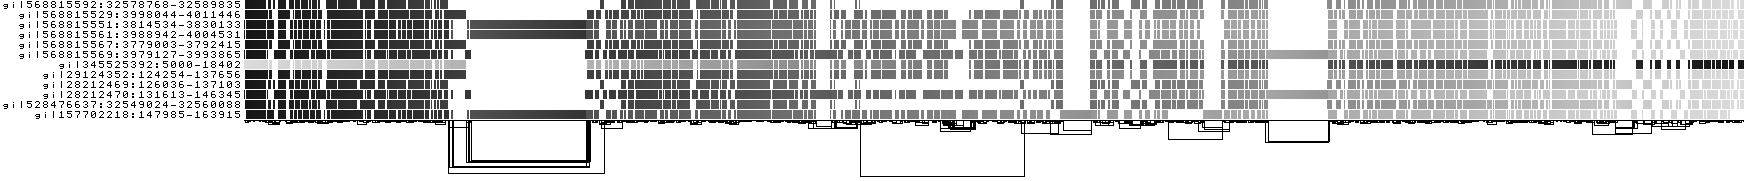
\includegraphics[width=\linewidth]{fig/latent_graph_structure/DRB1-3123.fa.gz.c666522.417fcdf.seqwish.og.YH.og.ud.png}
		\label{fig:ref_pos}
	\end{subfigure}
		\begin{subfigure}[t]{0.8\textwidth}
		\centering
		\caption{}
		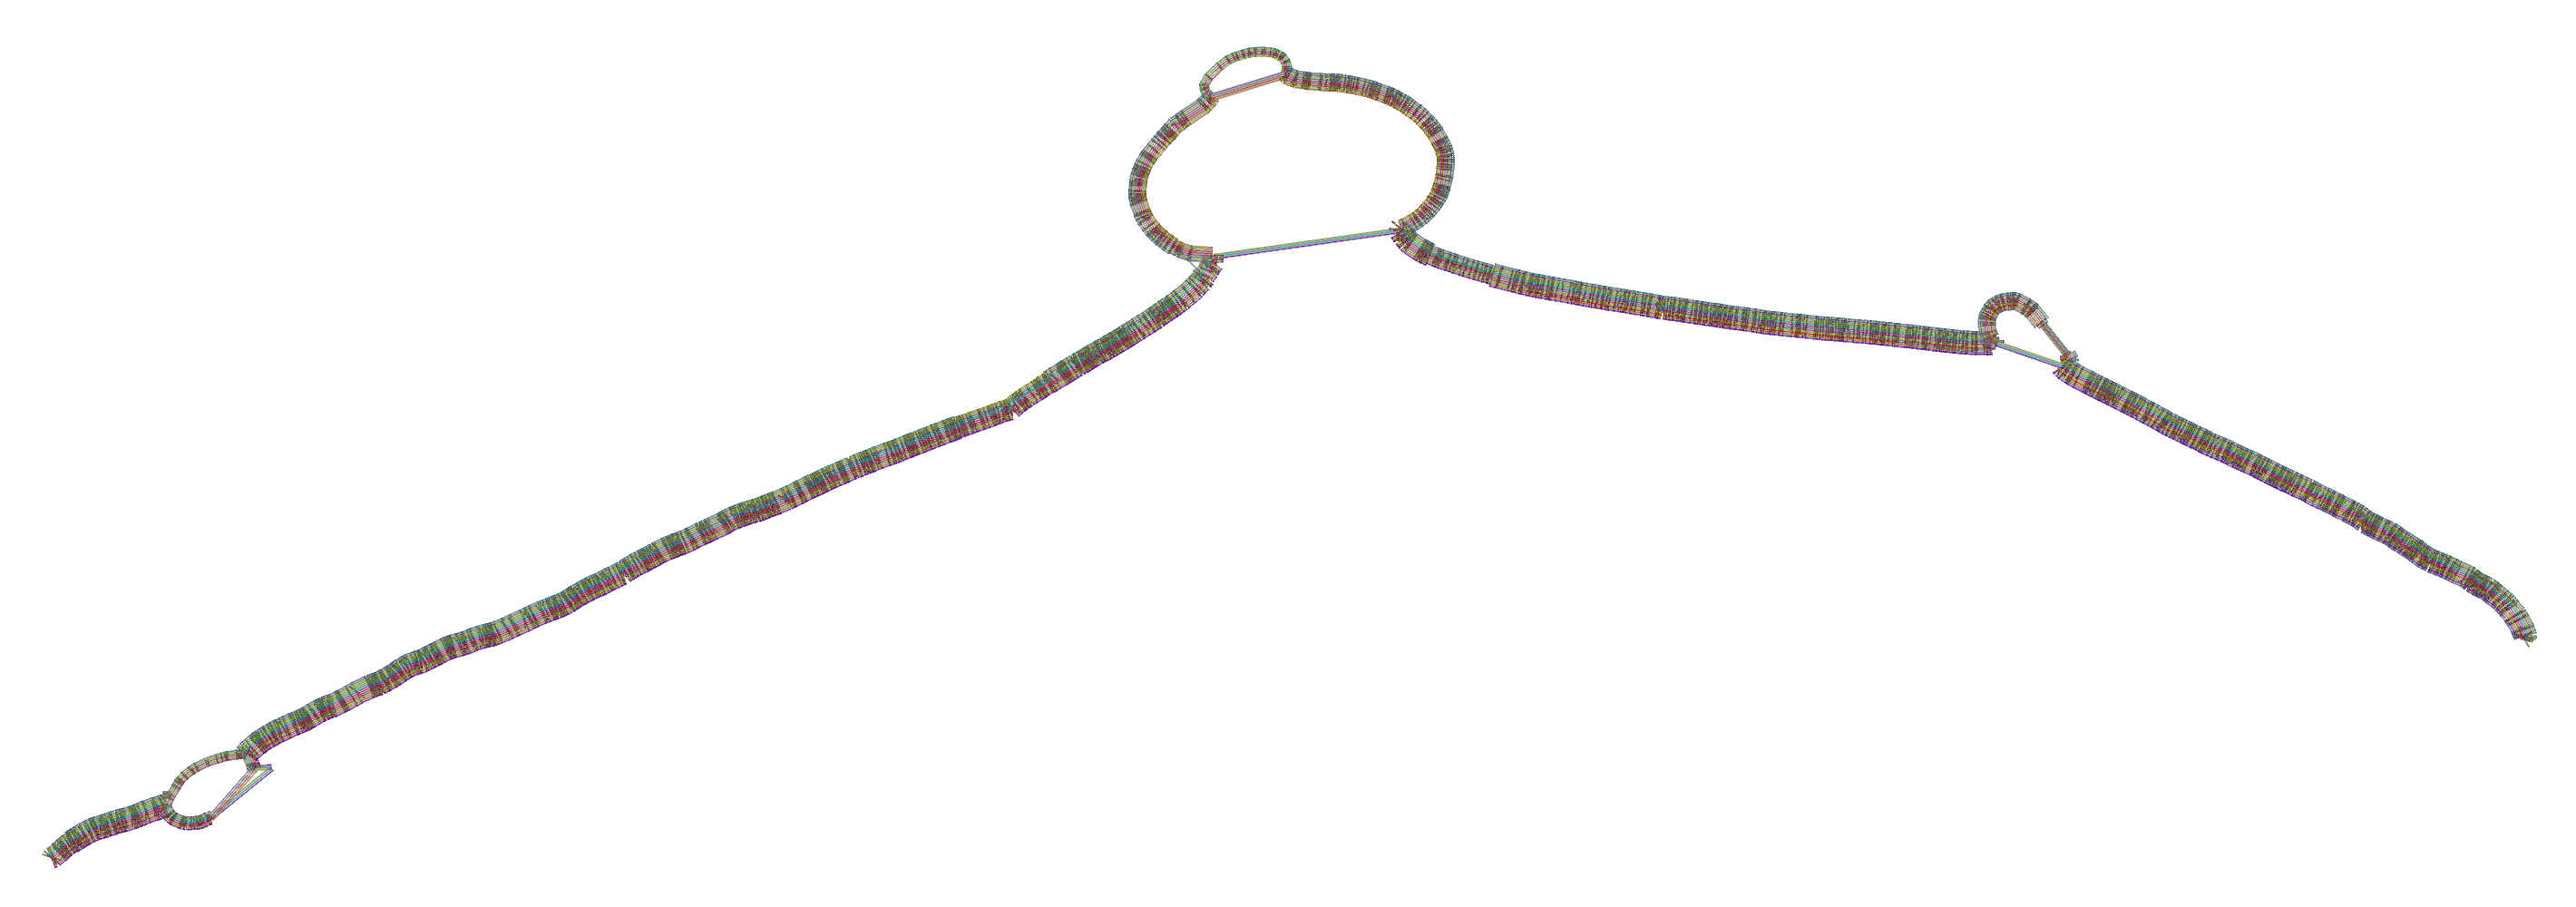
\includegraphics[width=\linewidth]{fig/latent_graph_structure/TODO_2d.png}
		\label{fig:2d}
	\end{subfigure}
	\caption{
		Latent graph structures.
		\textbf{(a)} Randomly sorted graph. \textbf{(b)} Randomly sorted graph by position. \textbf{(c)} PG-SGD sorted graph. \textbf{(d)} PG-SGD sorted graph by position. \textbf{(e)} Ygs sorted graph. \textbf{(f)} Ygs sorted graph by position. \textbf{(g)} Reference sorted graph. \textbf{(h)} Reference sorted graph by position. \textbf{(i)} 2D layout of graph.
	}
	\label{fig:latent_graph_structure}
\end{figure*}
    % Table 2: Metrics of the sorted graphs in Fig. 3.
    % \begin{table}[]
	\caption{Metrics of the latent graphs.}
	\begin{tabular}{|l|l|l|l|l|}
		\hline
		& RANDOM & Y & Ygs & Ref \\ \hline
		METRIC 1 &        &   &     &     \\ \hline
		METRIC 2 &        &   &     &     \\ \hline
	\end{tabular}
\end{table}
    % \paragraph{Bonus Section}
    % Fig. 4: Detect tension. Relax a graph. Detect tension afterwards.
    % I need to test this on a new data set I got from Erik.
    % I need to establish a fixed lower boundary for the tension from which on we don't relax anymore. \\
    % With a high quality layout, we can measure the discrepancy of the path layout position versus the expected path nucleotide position, the “tension” of a graph.
    % The greater the “tension”, the greater is the possibility of a biologically meaningless alignment.
    % This allows us to detect telomere collapsing alignment errors and hopefully (pangenome) assembly errors, subsequently correcting them.
    % \begin{figure*}[!htb]
	\centering
	%\hline
	\begin{subfigure}[t]{0.4\textwidth}
		\centering
		\caption{}
		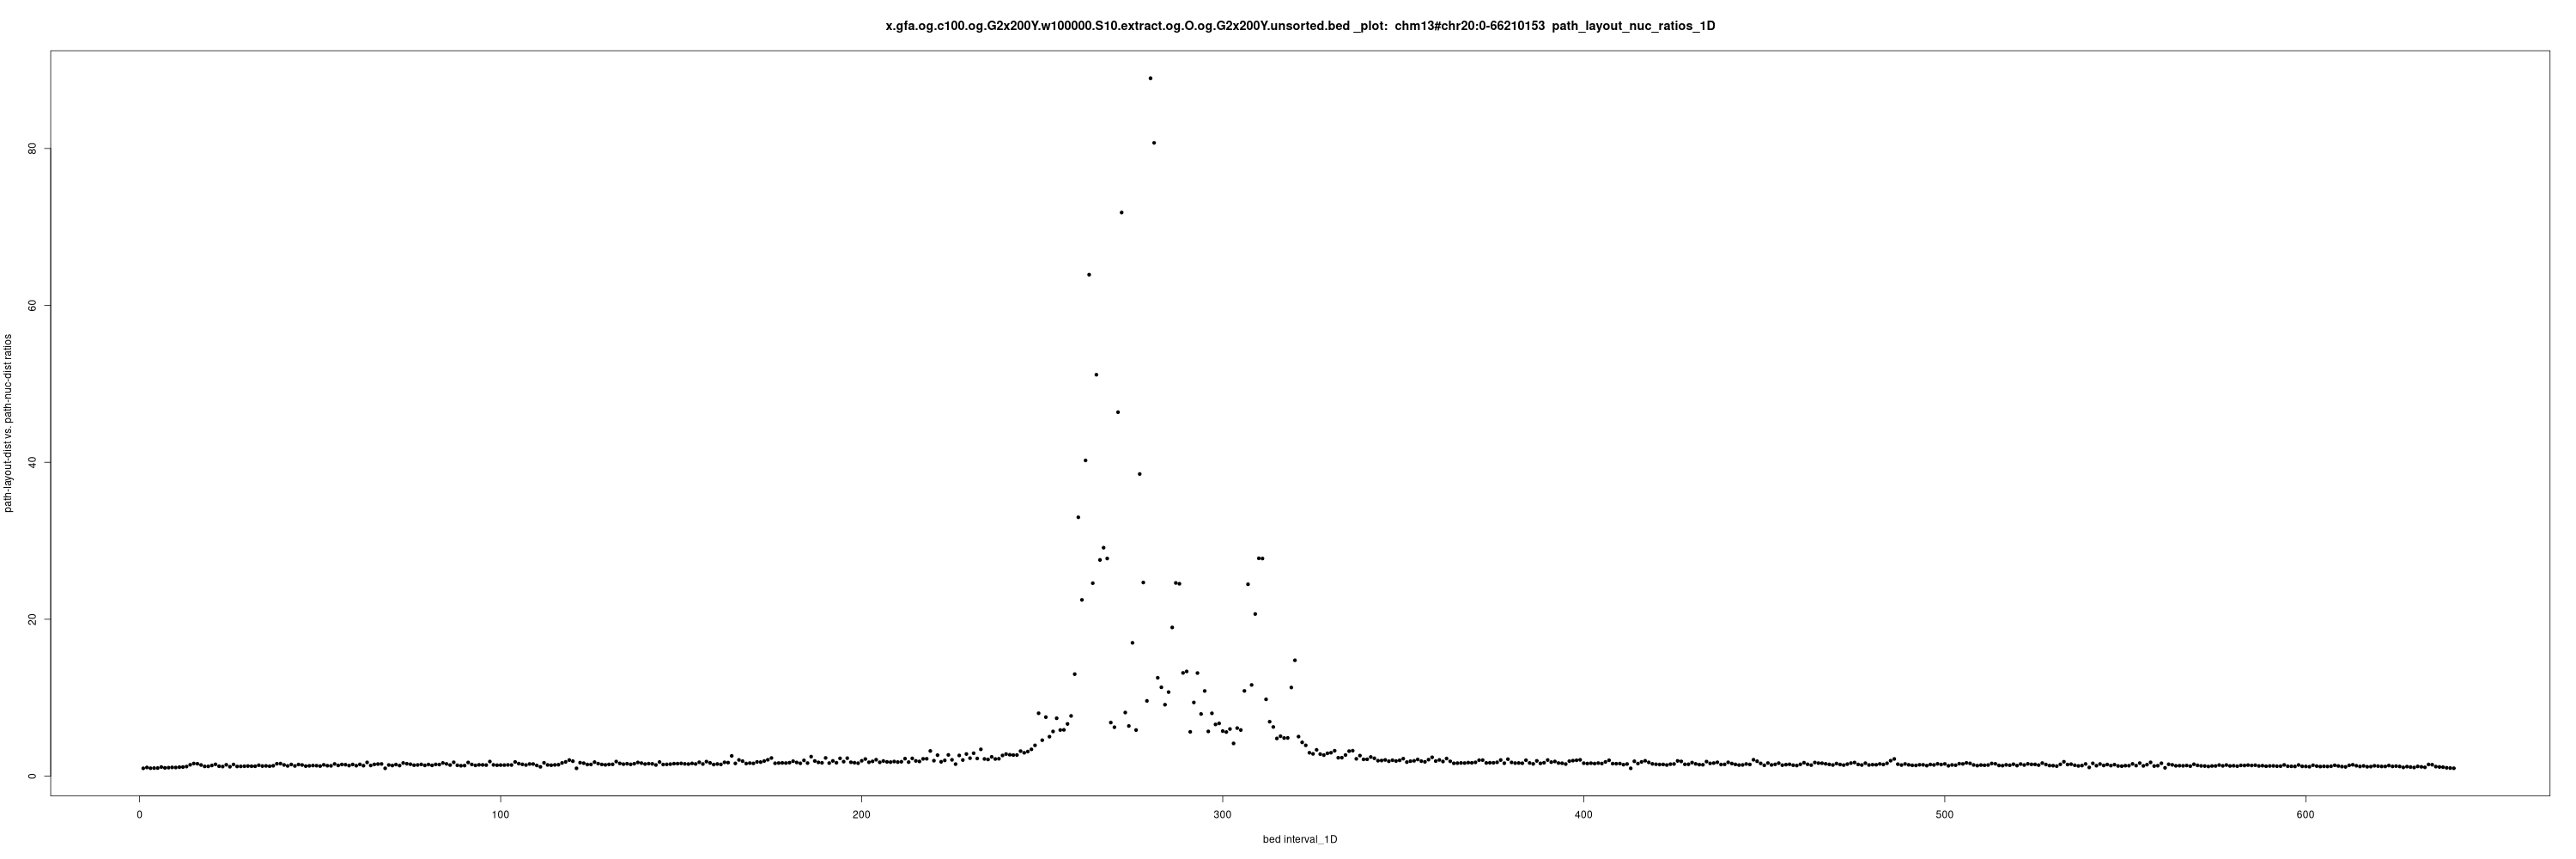
\includegraphics[width=\linewidth]{fig/tension/tension_bed.png}
		\label{fig:tension_bed}
	\end{subfigure}
	\begin{subfigure}[t]{0.4\textwidth}
		\centering
		\caption{}
		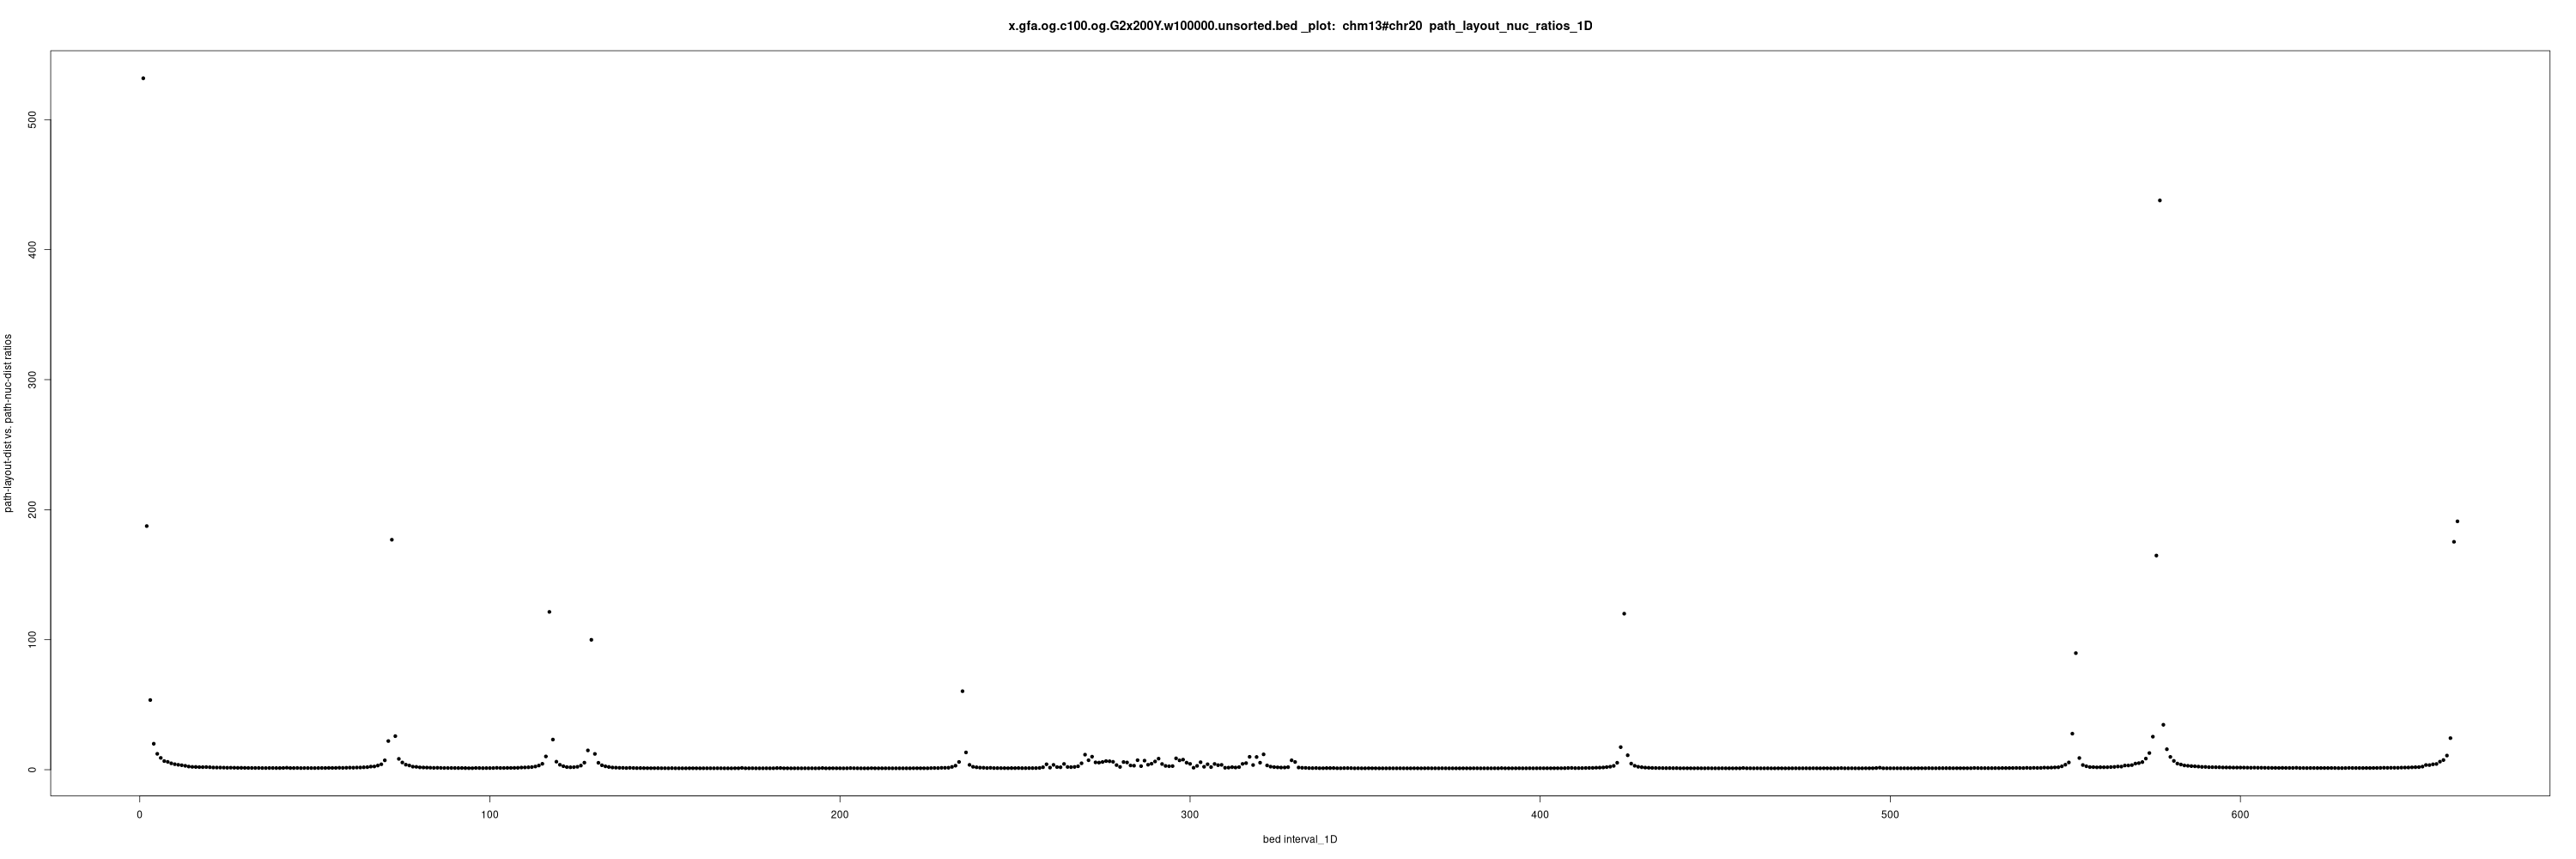
\includegraphics[width=\linewidth]{fig/tension/tension_bed_relaxed.png}
		\label{fig:tension_extracted}
	\end{subfigure}
\\
	%\smallskip
	\begin{subfigure}[t]{0.1\textwidth}
		\centering
		\caption{}
		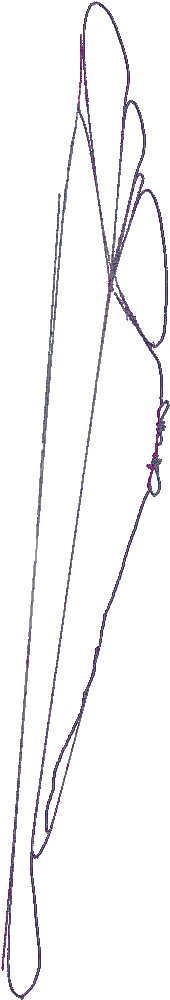
\includegraphics[width=\linewidth]{fig/tension/layout.png}
		\label{fig:tension_draw}
	\end{subfigure}
	\begin{subfigure}[t]{0.1\textwidth}
		\centering
		\caption{}
		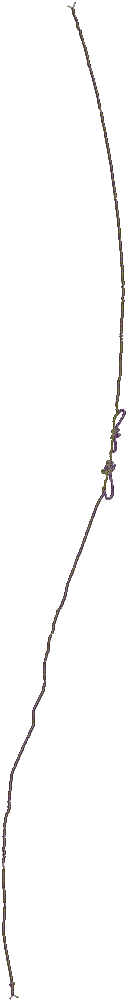
\includegraphics[width=\linewidth]{fig/tension/layout_relaxed.png}
		\label{fig:tension_draw_extracted}
	\end{subfigure}
	\caption{
		Detecting tension and relaxing a pangenome graph.
		\textbf{(a)} Tension detection before relaxation. \textbf{(b)} Tension detection after relaxation. \textbf{(c)} Folded 2D before relaxation. \textbf{(d)} Linearized 2D after relaxation.
	}
	\label{fig:tension}
\end{figure*}
    % \fi

	\section{Discussion}
	\label{sec:discussion}
	
	We presented Path-Guided Stochastic Gradient Descent (PG-SGD), the first layout algorithm for pangenome graphs that leverages the biological information available within the genomes represented in the graph.
	Our implementation efficiently computes the layout of pangenome graphs representing thousands of whole genomes.
	
	Graph visualization is key for understanding genome variations and the large-scale layouts produced by PG-SGD offer an unprecedented high-level perspective on variation in pangenomes.
	We implemented PG-SGD to generate layouts in 1 and 2 dimensions.
	These graph projections have already been employed in constructing and analyzing the first draft human pangenome reference \citep{Liao2023}, as well as in the discovery of heterologous recombination of human acrocentric chromosomes \citep{Guarracino2023}.
	Furthermore, they are applied in the creation and analysis of pangenome graphs for any species \citep{Guarracino2022, Garrison2023}.
	%The graph simplification pipeline smoothxg runs POA for each block of paths that are co-linear within each seqwish induced variation graph.
	%A prerequisite is that the graph nodes are sorted according to their occurrence in the graph's embedded paths.
	%Our 1D path-guided SGD algorithm is designed to provide this kind of sort.
	Of note, there still remains a gap in interactive and scalable solutions that merge layouts of large pangenome graph with annotation.
	Our algorithm will be the foundation of new pangenome graph browsers for studying graph layouts and the genome variation they represent (\url{https://github.com/chfi/waragraph}).
	
	\FIXME{@Jiajie + Niklas: just 2/3 sentences about going GPU?}

	PG-SGD can be extended to any number of dimensions.
	It can be seen as a graph embedding algorithm that converts high-dimensional, sparse pangenome graphs into low-dimensional, dense, and continuous vector spaces, while preserving its biologically relevant information.
	This enables the application of machine learning algorithms that use the graph layout for variant detection and classification. 
	Our future research involves leveraging these graph projections to detect structural variants and to identify and correct assembly errors
	Moreover, we are considering extending the algorithm to RNA and protein sequences to support pantranscriptome graphs \citep{sibbesen_haplotype-aware_2023} and panproteome graphs \citep{dabbaghie_panpa:_2023}, respectively.
	%Helpful could be to integrate more layout objectives \citep{ahmed_multicriteria_2021} like neighborhood preservation.

	\section*{Acknowledgments}
	
	%We are grateful to members of the HGSVC and HPRC production teams for their development of resources used in our exposition.
	%We thank the authors of the pangenome resources made available on GenBank which have made our experiments possible.
	A special thanks goes to Matthias Seybold from the Quantitative Biology Center for maintaining the Core Facility Cluster.
	
	\section*{Funding}
	
	S.H. acknowledges funding from the Central Innovation Programme (ZIM) for SMEs of the Federal Ministry for Economic Affairs and Energy of Germany.
	S.N. acknowledges Germany’s Excellence Strategy (CMFI), EXC-2124 and (iFIT)—EXC 2180–390900677.
	This work was supported by the BMBF-funded de.NBI Cloud within the German Network for Bioinformatics Infrastructure (de.NBI) (031A532B, 031A533A, 031A533B, 031A534A, 031A535A, 031A537A, 031A537B, 031A537C, 031A537D and 031A538A).
	A.G. acknowledges efforts by Nicole Soranzo to establish a pangenome research unit at the Human Technopole in Milan, Italy.
	JNM.S., J.L., and Z.Z. acknowledge funding from the NSF PPoSS Award \#2118709.
	
	\section*{Competing interests}
	The authors declare that they have no competing interests.
	
	\section*{Data availability}
	
	Code and links to data resources used to build this manuscript and its figures can be found in the paper's public repository: \url{https://github.com/pangenome/sorting-paper}.
		
	\bibliographystyle{natbib}
	
	\bibliography{document}
	
	\begin{appendices}
	    \section{Supplementary data}
	    %\FIXME{@ANDREA: Please add some more details about your clever quantization. Why. How. Where. When. Secs.} \\
	    %\FIXME{PGR-TK Paper - Layouts of challenging regions of the human pangenome. - https://www.nature.com/articles/s41592-023-01914-y} \\
		\FIXME{ADD LINKS TO OUR ANIMATIONS ON ZENODO} \\
	    \FIXME{From 1D layout to 1D node order} \\
	    \FIXME{reference-guided path-guided stochastic gradient descent}
	    \subsection{Performance evaluation}
	    \label{sec:performance}
	    \begin{table*}[!ht]
	\centering
	\ra{1.2}
	\caption{\label{tab:layout} Performance evaluation of computing a 2D layout of all chromosomal HPRC pangenome graphs. From GFA to the actual layout.}
	\begin{tabular}{@{}lrrrrrrrrr@{}}
		& & & & & &  \multicolumn{2}{c}{$\mathbf{time\ in\ minutes}$}  & \multicolumn{2}{c}{$\mathbf{memory\ in\ gigabytes}$}\\ \cmidrule(lr){7-8} \cmidrule(lr){9-10}
		{$\mathbf{name}$} & {$\mathbf{len}$} & {$\mathbf{nodes}$} & {$\mathbf{edges}$} & {$\mathbf{paths}$} & {$\mathbf{steps}$} & {$\mathbf{pg-sgd}$} & {$\mathbf{bng}$} & {$\mathbf{pg-sgd}$} & {$\mathbf{bng}$}\\ \hline
		chr1 & 1.12e+09 & 1.11e+07 & 1.54e+07 & 2.26e+03 & 6.01e+08 & \textbf{68} & 1427 & \textbf{56.00} & 195.33 \\ 
		chr2 & 3.47e+08 & 6.68e+06 & 9.27e+06 & 1.65e+03 & 3.89e+08 & \textbf{47} & 521 & \textbf{37.29} & 81.97 \\ 
		chr3 & 4.06e+08 & 6.20e+06 & 8.62e+06 & 1.56e+03 & 4.55e+08 & \textbf{52} & 481 & \textbf{41.71} & 93.83 \\ 
		chr4 & 2.73e+08 & 5.91e+06 & 8.23e+06 & 1.35e+03 & 4.97e+08 & \textbf{56} & 423 & \textbf{45.02} & 79.48 \\ 
		chr5 & 3.35e+08 & 5.39e+06 & 7.51e+06 & 1.20e+03 & 4.04e+08 & \textbf{46} & 375 & \textbf{36.48} & 75.10 \\ 
		chr6 & 2.29e+08 & 4.70e+06 & 6.56e+06 & 1.41e+03 & 4.03e+08 & \textbf{46} & 271 & \textbf{37.22} & 71.26 \\ 
		chr7 & 2.71e+08 & 5.17e+06 & 7.25e+06 & 1.22e+03 & 4.10e+08 & \textbf{46} & 346 & \textbf{37.88} & 73.81 \\ 
		chr8 & 1.93e+08 & 4.26e+06 & 5.95e+06 & 8.55e+02 & 4.29e+08 & \textbf{47} & 233 & \textbf{38.07} & 54.70 \\ 
		chr9 & 1.01e+09 & 8.80e+06 & 1.23e+07 & 8.67e+02 & 3.31e+08 & \textbf{38} & 957 & \textbf{31.79} & 131.96 \\ 
		chr10 & 2.56e+08 & 4.50e+06 & 6.26e+06 & 8.79e+02 & 2.72e+08 & \textbf{32} & 260 & \textbf{25.25} & 67.87 \\ 
		chr11 & 2.83e+08 & 4.73e+06 & 6.54e+06 & 6.53e+02 & 2.38e+08 & \textbf{28} & 286 & \textbf{21.77} & 68.54 \\ 
		chr12 & 2.44e+08 & 4.10e+06 & 5.71e+06 & 7.68e+02 & 2.54e+08 & \textbf{27} & 206 & \textbf{23.99} & 51.22 \\ 
		chr13 & 3.47e+08 & 4.34e+06 & 6.08e+06 & 2.58e+03 & 3.12e+08 & \textbf{34} & 237 & \textbf{28.64} & 85.85 \\ 
		chr14 & 2.73e+08 & 4.15e+06 & 5.79e+06 & 1.82e+03 & 2.62e+08 & \textbf{28} & 222 & \textbf{24.17} & 78.13 \\ 
		chr15 & 5.64e+08 & 5.20e+06 & 7.26e+06 & 2.06e+03 & 4.02e+08 & \textbf{35} & 334 & \textbf{35.69} & 102.97 \\ 
		chr16 & 3.39e+08 & 3.91e+06 & 5.53e+06 & 1.52e+03 & 6.91e+08 & 512 & \textbf{244} & 61.02 & \textbf{53.00} \\ 
		chr17 & 1.73e+08 & 2.76e+06 & 3.93e+06 & 1.42e+03 & 3.25e+08 & \textbf{33} & 102 & \textbf{28.69} & 49.50 \\ 
		chr18 & 2.44e+08 & 2.83e+06 & 3.98e+06 & 1.27e+03 & 3.00e+08 & \textbf{31} & 106 & \textbf{26.78} & 45.01 \\ 
		chr19 & 2.91e+08 & 3.02e+06 & 4.21e+06 & 1.07e+03 & 2.03e+08 & \textbf{21} & 117 & \textbf{18.43} & 40.18 \\ 
		chr20 & 1.87e+08 & 2.82e+06 & 3.97e+06 & 8.24e+02 & 2.35e+08 & \textbf{25} & 108 & \textbf{21.04} & 39.05 \\ 
		chr21 & 2.74e+08 & 2.76e+06 & 3.88e+06 & 3.03e+03 & 2.21e+08 & \textbf{23} & 103 & \textbf{19.12} & 46.47 \\ 
		chr22 & 4.64e+08 & 3.76e+06 & 5.22e+06 & 1.76e+03 & 2.05e+08 & \textbf{22} & 183 & \textbf{18.65} & 45.13 \\ 
		chrX & 2.07e+08 & 3.46e+06 & 4.89e+06 & 2.42e+03 & 2.70e+08 & \textbf{28} & 155 & \textbf{24.84} & 43.05 \\ 
		chrY & 8.80e+07 & 3.18e+05 & 4.41e+05 & 3.07e+02 & 1.34e+07 & \textbf{1} & 5 & \textbf{1.57} & 4.65 \\ 
		chrM & 1.76e+04 & 1.40e+03 & 1.89e+03 & 4.40e+01 & 4.06e+04 & \textbf{1} & \textbf{1} & 0.49 & \textbf{0.04}  \\ 
		all chrs & 8.42e+09 & 1.11e+08 & 1.55e+08 & 3.48e+04 & 8.12e+09 & \textbf{1020} & ?  & \textbf{738.76} & ? ($\approx$1567.45)\\
		\bottomrule
	\end{tabular}
\end{table*}
		\subsection{Graph layouts}
		\FIXME{chr1}
		\FIXME{chr2}
		\FIXME{...}
		\FIXME{FIGURE WITH ALL CHROMOSOMES TOGETHER}
	\end{appendices}

\end{document}
